% !TEX encoding = UTF-8 Unicode 
% !TEX root = praca.tex

\chapter*{Metodyka badań}

\section*{Plan badań}

\begin{enumerate}
	\item \textbf{Skonfigurowanie środowiska pracy}, w tym odpowiednie biblioteki Pythona.
	\item \textbf{Załadowanie zbioru danych}, który będzie używany do testowania metod wyjaśniania XAI.
	\item \textbf{Dobór parametrów}:
	      \begin{itemize}
		      \item Określenie optymalnych wartości parametrów dla każdej z metod wyjaśniania.
	      \end{itemize}
	\item \textbf{Wygenerowanie wyjaśnień}:
	      \begin{itemize}
		      \item Wygenerowanie wyjaśnień dla wszystkich obrazów ze zbioru danych za pomocą wybranych metod XAI i odpowiednich parametrów.
		      \item Zapisanie uzyskanych wyjaśnień w celu dalszej analizy.
	      \end{itemize}
	\item \textbf{Analiza spójności wyjaśnień}
	\item \textbf{Wykonanie podstawowych badań na wszystkich obrazach}:
	      \begin{itemize}
		      \item Zastosowanie wybranych miar jakości, w celu oceny i analizy skuteczności każdej metody wyjaśniania.
	      \end{itemize}
	\item \textbf{Wykonanie badań grupując wyjaśnienia na kategorie obrazów}:
	      \begin{itemize}
		      \item Analiza skuteczności metod wyjaśniania dla poszczególnych kategoriach obrazów i porównanie wyników.
	      \end{itemize}
	\item \textbf{Wykonanie badań grupując na wielkość obiektu}:
	      \begin{itemize}
		      \item Analiza skuteczności metod wyjaśniania dla pogrupowanych wielkością obiektów obrazów i porównanie wyników.
	      \end{itemize}

	\item \textbf{Połączenie wyjaśnień wygenerowanych przez różne metody XAI}:
	      \begin{itemize}
		      \item Połączenie wygenerowanych wyjaśnień
		      \item Wykonanie podstawowych badań na wszystkich obrazach z użyciem połączonych wyjaśnień
	      \end{itemize}
\end{enumerate}

\section*{Przygotowanie środowiska}

Do przeprowadzenia eksperymentów z wybranymi metodami XAI wymagane było odpowiednie przygotowanie środowiska programistycznego.
W tej pracy wykorzystano  następujące narzędzia i biblioteki:
\begin{itemize}
	\item \textbf{Python}\cite{python} - wysokopoziomowy język programowania, który jest szeroko stosowany w dziedzinie nauki o danych i uczenia maszynowego.
	      Był to główny język używany w badaniach.
	\item \textbf{TensorFlow}\cite{tensorflow} - popularna biblioteka open-source do uczenia maszynowego, która jest szeroko stosowana w dziedzinie uczenia maszynowego do tworzenia i trenowania modeli głębokich.
	\item \textbf{LIME}\cite{limedoc} - biblioteka do generowania lokalnie interpretowalnych wyjaśnień dla decyzji modelu.
	\item \textbf{SHAP}\cite{shapdoc} - biblioteka oparta na teorii gier, która oblicza wartości Shapleya, określająca wpływ poszczególnych cech na wynik modelu.
	\item \textbf{numpy}\cite{numpy} - szeroko stosowana biblioteka do obliczeń numerycznych.
	\item \textbf{matplotlib}\cite{matplotlib} - biblioteka do tworzenia wykresów i wizualizacji danych, szeroko stosowana w dziedzinie uczenia maszynowego.
	\item \textbf{scikit-image}\cite{scikitimage} - biblioteka do przetwarzania obrazów, która zawiera wiele funkcji do przetwarzania obrazów.
	\item \textbf{Pandas}\cite{pandas} - biblioteka do manipulacji i analizy danych, które oferuje struktury danych hi narzędzia do przetwarzania danych tabelarycznych.
	      Szczególnie użyteczna do zarządzania i analizowania zbiorów danych używanych w badaniach.
	\item \textbf{seabron}\cite{seaborn} - biblioteka do tworzenia wykresów i wizualizacji danych, współgrająca z biblioteką pandas
\end{itemize}

Środowisko to pozwoliło na tworzenie i analizowanie wyjaśnień dla już istniejących modeli głębokiego uczenia.
Narzędzia te umożliwiły także wizualizację wyników, co było kluczowe dla zrozumienia i prezentacji działania zastosowanych metod XAI.

\section*{Wybór bazy obrazów}

W tej pracy wykorzystano bazę danych \textbf{ImageNet-9}\cite{imagenet} jest to podzbiór ImageNet, najpopularniejszej bazy zdjęć.
Podzbiór ten zawiera zawiera 9 kategorii, z których każda posiada 450 obrazów.
Ważnym aspektem wyboru tego zbioru były oznaczone obszary obiektów klasyfikowanych, co pozwalało na posiadanie wiedzy o ważnych obszarach, która została użyta do oceny jakości generowanych wyjaśnień.
Kategorie obejmowały:
\begin{enumerate}
	\item Pies (dog)
	\item Ptak (bird)
	\item Pojazd na kołach (wheeled vehicle)
	\item Gad (reptile)
	\item Mięsożerca (carnivore)
	\item Insekt (insect)
	\item Instrument muzyczne (musical instrument)
	\item Naczelny (primate)
	\item Ryba (fish)
\end{enumerate}

Dodatkowo baza obrazów została podzielona ze względu na wielkość obiektu, jaki procent obrazu zajmuje obiekt docelowy.
Podzielony został na 5 kategorie obrazów:
\begin{itemize}
	\item Bardzo mały (XS) - obiekt zajmuje mniej niż 2\% obrazu. W tej kategorii znajduje się 129 obrazów.
	\item Mały (S) - obiekt zajmuje mniej niż 25\%, ale więcej niż 2\% obrazu. W tej kategorii znajduje się 3912 obrazów.
	\item Średni (M) - obiekt zajmuje mniej niż 50\%, ale więcej niż 25\% obrazu. W tej kategorii znajduje się 4311 obrazów.
	\item Duży (L) - obiekt zajmuje mniej niż 90\%, ale więcej niż 50\% obrazu. W tej kategorii znajduje się 3657 obrazów.
	\item Bardzo duży (XL) - obiekt zajmuje więcej niż 90\% obrazu. W tej kategorii znajduje się 141 obrazów.
\end{itemize}

Przykłady obrazów dla kategorii wielkości zostały przedstawione na Rys \ref{rys:examples_size_cat}.

\begin{figure}[h]
	\centering
	\begin{subfigure}[b]{0.3\textwidth}
		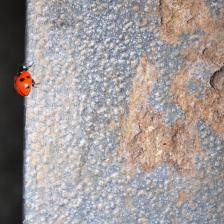
\includegraphics[width=.9\textwidth]{img/examples/size_category_verysmall}
		\caption{Bardzo mały obiekt (0.7553\%)}  \label{}
	\end{subfigure}
	\begin{subfigure}[b]{0.3\textwidth}
		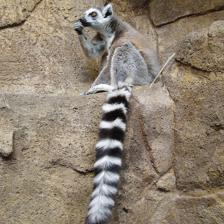
\includegraphics[width=.9\textwidth]{img/examples/size_category_small}
		\caption{Mały obiekt (13.7915\%)}  \label{}
	\end{subfigure}
	\begin{subfigure}[b]{0.3\textwidth}
		\centering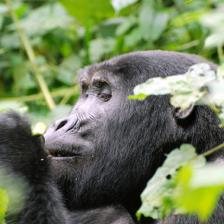
\includegraphics[width=.9\textwidth]{img/examples/size_category_medium}
		\caption{Średni obiekt (49.1510\%)}  \label{}
	\end{subfigure}
	\begin{subfigure}[b]{0.3\textwidth}
		\centering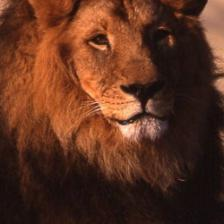
\includegraphics[width=.9\textwidth]{img/examples/size_category_big}
		\caption{Duży obiekt (66.5577\%)}  \label{}
	\end{subfigure}
	\begin{subfigure}[b]{0.3\textwidth}
		\centering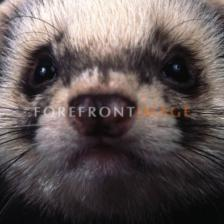
\includegraphics[width=.9\textwidth]{img/examples/size_category_verybig}
		\caption{Bardzo duży obiekt (90.2224\%)}  \label{}
	\end{subfigure}
	\caption{Przykłady obrazów dla różnych kategorii wielkości}
	\label{rys:examples_size_cat}
\end{figure}

\section*{Wybór parametrów metod XAI}
Wybór odpowiednich parametrów jest kluczowym etapem w procesie tworzenia i oceny modeli głębokiego uczenia oraz metod wyjaśnialnej sztucznej inteligencji (XAI).
Parametry mają bezpośredni wpływ na jakość, dokładność i interpretowalność wyników generowanych przez modele i metody XAI.
W tej sekcji omówione zostało, jakie parametry zostały wybrane dla każdej z zastosowanych metod (LIME, SHAP i GradCAM) oraz jak te parametry wpływają na wyniki i interpretacje uzyskane w badaniach

\subsection*{LIME}
W celu porównania metod na większej liczbie obrazów konieczne było ustalenie wartości parametrów dla poszczególnych technik.
W bibliotece LIME używamy tych parametrów LIME:
\begin{itemize}
	\item \textbf{num samples}
	\item \textbf{num features}
	\item \textbf{possitive only}
	\item \textbf{min weight}
\end{itemize}

Parametr \textbf{'num\_samples'} to liczba próbek generowanych wokół wyjaśnianej instancji.
Wyjaśnienia LIME opierają się na lokalnych modelach zastępczych, które są trenowane na perturbowanych wersjach oryginalnych danych wejściowych.
Zbyt mała liczba próbek może prowadzić do niedokładnych wyjaśnień, ponieważ lokalny model zastępczy może nie być w stanie prawidłowo uchwycić istotnych wzorców w danych.
Z drugiej strony, zbyt duża liczba próbek może prowadzić do znacznych kosztów obliczeniowych, co wydłuża czas potrzebny na wygenerowanie wyjaśnień.
W tej pracy użyto wartości num\_samples=1000, co stanowi kompromis między dokładnością wyjaśnień a kosztami obliczeniowymi.

\begin{figure}[h]
	\centering
	\begin{subfigure}[b]{0.3\textwidth}
		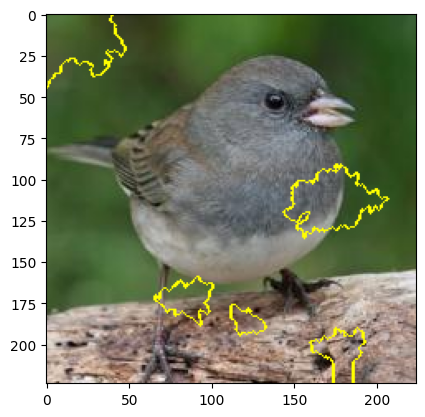
\includegraphics[width=.9\textwidth]{img/parameters/lime/num_samples_5}
		\caption{num\_samples=5}  \label{rys:parameters_lime_numsamples_5}
	\end{subfigure}
	\begin{subfigure}[b]{0.3\textwidth}
		\centering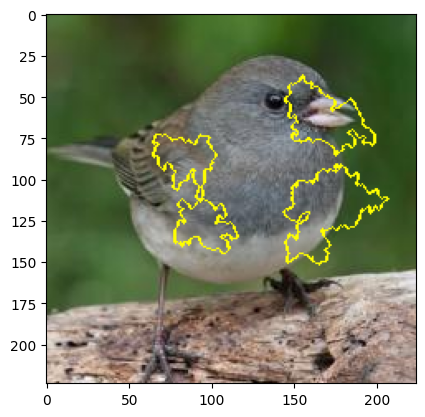
\includegraphics[width=.9\textwidth]{img/parameters/lime/num_samples_1000}
		\caption{num\_samples 1000}  \label{rys:parameters_lime_numsamples_1000}
	\end{subfigure}
	\begin{subfigure}[b]{0.3\textwidth}
		\centering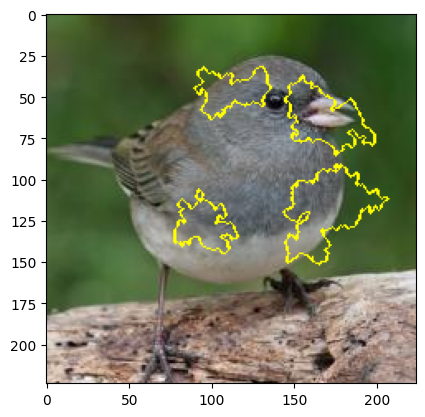
\includegraphics[width=.9\textwidth]{img/parameters/lime/num_samples_5000}
		\caption{num\_samples 5000}  \label{rys:parameters_lime_numsamples_5000}
	\end{subfigure}
	\caption{Przykłady wyjaśnień LIME dla różnych wartości num\_samples}
\end{figure}

Parametr \textbf{'num\_features'} oznacza maksymalną ilość cech które mogą występować w wyjaśnieniu.
Wyjaśnienia LIME polegają na identyfikacji najważniejszych cech, które wpływają na decyzję modelu w danym punkcie.
W przypadku obrazów, cech te są reprezentowane przez super-piksele, czyli segmenty obrazu zawierające grupy pikseli.
Określenie zbyt niskiej wartości dla num\_features może prowadzić do pominięcia istotnych cech, co skutkuje niepełnym wyjaśnieniem.
Z kolei zbyt wysoka wartość może sprawić, że wyjaśnienie będzie zawierało nadmiarowe informacje, które mogą być trudne do interpretacji.

W przypadku tej pracy, użyto wysokiej wartości (num\_features = 100000), aby zapewnić, że wszystkie potencjalnie ważne cechy zostaną uwzględnione w wyjaśnieniach niezależnie od wielkości obiektu.

\begin{figure}[h]
	\centering
	\begin{subfigure}[b]{0.3\textwidth}
		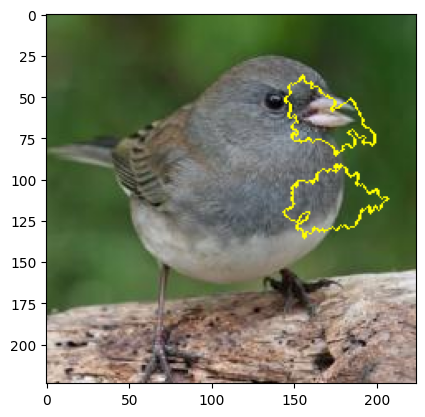
\includegraphics[width=.9\textwidth]{img/parameters/lime/num_features_2}
		\caption{num\_features 2}  \label{rys:parameters_lime_numsamples_5}
	\end{subfigure}
	\begin{subfigure}[b]{0.3\textwidth}
		\centering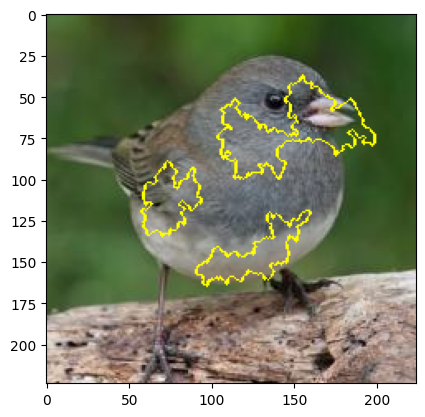
\includegraphics[width=.9\textwidth]{img/parameters/lime/num_features_100000}
		\caption{num\_features 100000}  \label{rys:parameters_lime_numsamples_1000}
	\end{subfigure}
	\caption{Przykłady wyjaśnień LIME dla różnych wartości num\_features}
\end{figure}

Parametr \textbf{min\_weight} określa minimalną wagę cech, która musi być spełniona, aby cecha była uwzględniona w wyjaśnieniu.
W tej pracy zostało ustawione min\_weight na 60\% największej wagi dla konkretnego wyjaśnienia, wagi cech mogą mieć bardzo różne wartości w różnych przypadkach.
Ustalenie stałej wartości prowadzi do sytuacji, w której w niektórych przypadkach żadna cecha nie zostałaby zaznaczona, a w innych wszystkie cechy byłby uwzględnione.

\begin{figure}[h]
	\centering
	\begin{subfigure}[b]{0.3\textwidth}
		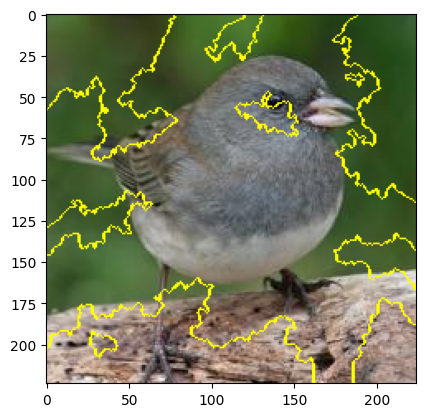
\includegraphics[width=.9\textwidth]{img/parameters/lime/min_weight_00}
		\caption{min\_weight = 0.0}  \label{rys:parameters_lime_numsamples_5}
	\end{subfigure}
	\begin{subfigure}[b]{0.3\textwidth}
		\centering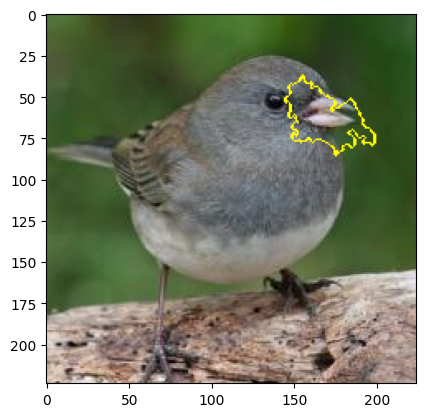
\includegraphics[width=.9\textwidth]{img/parameters/lime/min_weight_03}
		\caption{min\_weight = 0.3}  \label{rys:parameters_lime_numsamples_1000}
	\end{subfigure}
	\begin{subfigure}[b]{0.3\textwidth}
		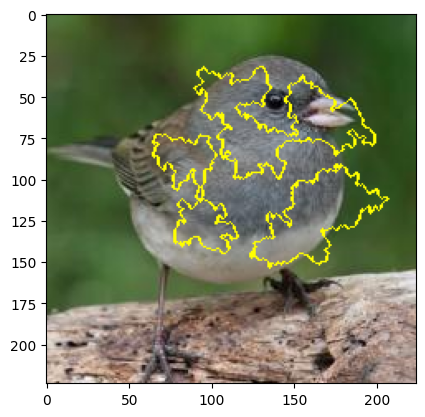
\includegraphics[width=.9\textwidth]{img/parameters/lime/min_weight_06m}
		\caption{min\_weight = 60\% wagi maksymalnej}  \label{rys:parameters_lime_numsamples_5}
	\end{subfigure}
	\caption{Przykłady wyjaśnień LIME dla różnych wartości min\_weight}
\end{figure}

Parametr \textbf{'positive\_only'} określa, czy wyjaśnienia powinny uwzględniać tylko cechy, które mają pozytywny wpływ na klasyfikację.
Ustawienie tego parametru na prawdziwy pomaga w identyfikowaniu pozytywnych cech, które wpływają na decyzję modelu.
Natomiast ustawienie tego parametru na prawdziwy pomaga w identyfikowaniu także negatywnych cech.
Ta praca skupia się na wyjaśnianiu dlaczego model podjął daną decyzję więc parametr positive\_only jest ustawiony na prawdziwy.


\subsection*{SHAP}
Analogicznie do metody LIME, musimy ustalić odpowiednie parametry dla metody SHAP.
Parametry mają kluczowe znaczenie dla uzyskania dokładnych i interpretowalnych wyjaśnień.
W przypadku metody SHAP, wybrano dwa główne parametry:
\begin{itemize}
	\item \textbf{max\_evals}
	\item \textbf{threshold}
\end{itemize}

Parametr \textbf{max\_evals} to liczba maksymalnych ewaluacji modelu, które mogą być wykonane w celu obliczenia wartości SHAP.
Wartość ta ma bezpośredni wpływ na jakość i dokładność wyjaśnień.
Wyższa liczba ewaluacji zazwyczaj prowadzi do bardziej precyzyjnych wyników, ponieważ pozwala na lepsze oszacowanie wpływu poszczególnych cech na wynik modelu.
Jednakże, zwiększenie wartości max\_evals wiąże się również ze zwiększonymi kosztami obliczeniowymi, co może być istotne przy analizie dużych zbiorów danych lub skomplikowanych modeli.

W tej pracy ustaliliśmy wartość max\_evals na 500, co stanowi kompromis pomiędzy dokładnością wyjaśnień a czasem potrzebnym na ich obliczenie.

\begin{figure}[h]
	\centering
	\begin{subfigure}[b]{0.45\textwidth}
		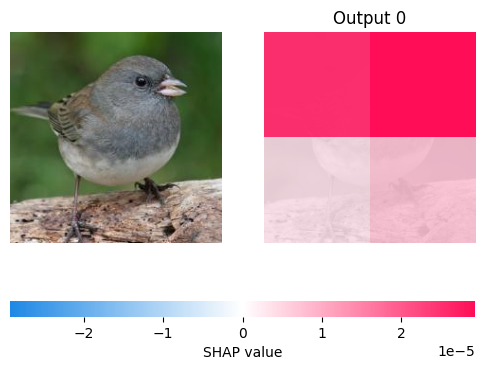
\includegraphics[width=.9\textwidth]{img/parameters/shap/max_evals_10}
		\caption{max\_evals 10}  \label{rys:parameters_lime_numsamples_5}
	\end{subfigure}
	\begin{subfigure}[b]{0.45\textwidth}
		\centering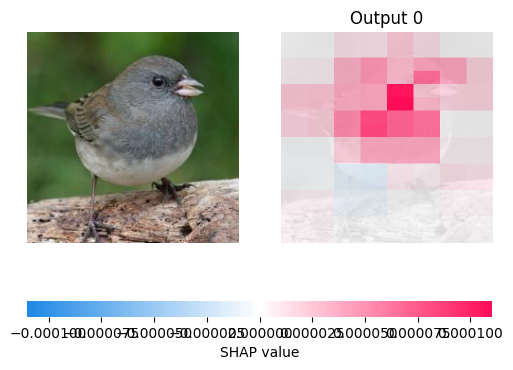
\includegraphics[width=.9\textwidth]{img/parameters/shap/max_evals_500}
		\caption{max\_evals 500}  \label{rys:parameters_lime_numsamples_1000}
	\end{subfigure}
	\caption{Przykłady wyjaśnienia SHAP dla parametru max\_evals}
\end{figure}
Parametr \textbf{threshold} określa minimalną wartość cechy, która musi być spełniona, aby cecha została uwzględniona w wyjaśnieniu.
Wartość progowa jest ważna, ponieważ pozwala na filtrowanie mniej istotnych cech, co może uprościć wyjaśnienia i uczynić je bardziej zrozumiałymi.
W przypadku obrazów, gdzie liczba cech jest bardzo duża, odpowiednie ustawienie tego parametru jest kluczowe.

W tej pracy ustaliliśmy wartość threshold jako 40\% maksymalnej wagi wyjaśnienia.
Parametr ten został stworzony, aby umożliwić porównywanie różnych metod wyjaśniania.
Threshold pełni kluczową rolę w procesie modyfikacji zbioru cech wyjaśnień.
Względem tego parametru, wybierane są tylko te cechy, których wartości są większe lub równe średniej wartości cech.
Dzięki temu mechanizmowi, wyjaśnienia koncentrują się na cechach, które mają znaczący wpływ na decyzję modelu, eliminując te, które mają minimalny wpływ.
W efekcie, wyjaśnienia stają się bardziej skoncentrowane na kluczowych cechach decyzyjnych.

\begin{figure}[h]
	\centering
	\begin{subfigure}[b]{0.45\textwidth}
		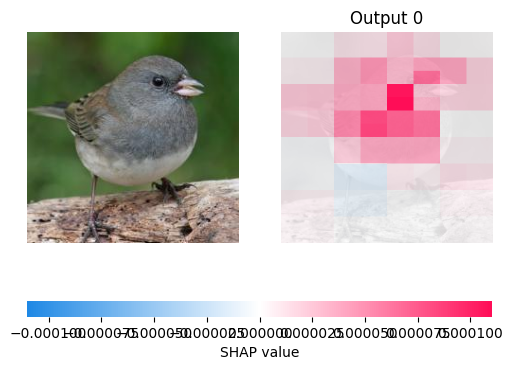
\includegraphics[width=.9\textwidth]{img/parameters/shap/threshold_base}
		\caption{Oryginalne wyjaśnienie}  \label{rys:parameters_lime_numsamples_5}
	\end{subfigure}
	\begin{subfigure}[b]{0.45\textwidth}
		\centering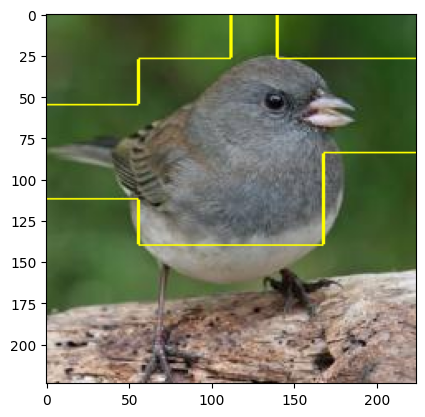
\includegraphics[width=.9\textwidth]{img/parameters/shap/threshold_mean}
		\caption{Zmodyfikowane wyjaśnienie}  \label{rys:parameters_lime_numsamples_1000}
	\end{subfigure}
	\caption{Przykład modyfikowania wyjaśnienia SHAP za pomocą threshold}
\end{figure}

\subsection*{GradCAM}
W przypadku metody GradCAM również musimy skonfigurować parametr "threshold", który pozwoli nam porównać różne wyjaśnienia generowane przez tę metodę.
Parametr ten jest istotny dla procesu modyfikacji wyjaśnień, podobnie jak miało to miejsce w przypadku metody SHAP.
Wartość "threshold" w metodzie GradCAM określa minimalną wartość pikseli, które będą uwzględnione w wyjaśnieniu.
Im wyższa wartość threshold, tym mniej pikseli zostanie uwzględnionych, co może prowadzić do bardziej skupionych wyjaśnień na kluczowych obszarach obrazu.
Z kolei niższa wartość threshold może uwzględnić więcej pikseli, co może prowadzić do bardziej rozproszonych wyjaśnień.

Wybrana została wartość threshold na poziomie 0.2.
\begin{equation}
	\hat{E} =  \{ e_i \in E \mid e_i \geq 0.2 \}
	\label{eq:modified_explanation_gradcam}
\end{equation}
Gdzie:
\begin{itemize}[label=]
	\item $\hat{E}$ to zbiór zmodyfikowanych wartości cech wyjaśnień
	\item $\text{E}$ to oryginalny zbiór wartości cech wyjaśnień
\end{itemize}

\begin{figure}[!h]
	\centering
	\begin{subfigure}[b]{0.9\textwidth}
		\centering
		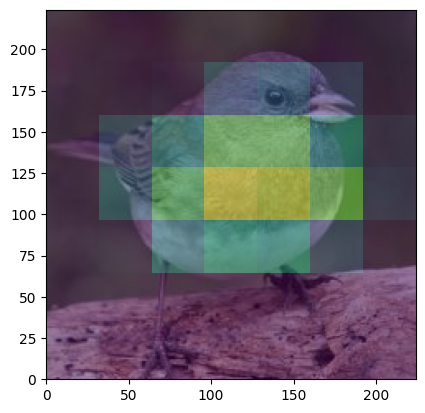
\includegraphics[width=.45\textwidth]{img/parameters/gradcam/threshold_base}
		\caption{Oryginalne wyjaśnienie}  \label{rys:parameters_lime_numsamples_5}
	\end{subfigure}
	\begin{subfigure}[b]{0.45\textwidth}
		\centering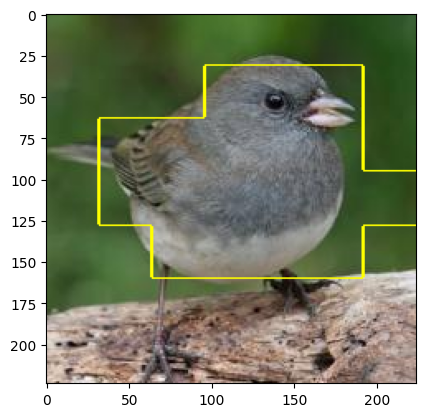
\includegraphics[width=.9\textwidth]{img/parameters/gradcam/threshold_01}
		\caption{Threshold 0.1}  \label{rys:parameters_lime_numsamples_1000}
	\end{subfigure}
	\begin{subfigure}[b]{0.45\textwidth}
		\centering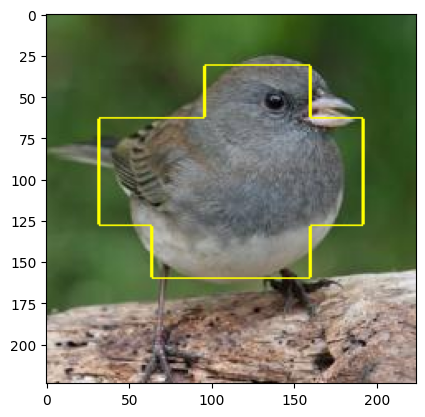
\includegraphics[width=.9\textwidth]{img/parameters/gradcam/threshold_02}
		\caption{Threshold 0.2}  \label{rys:parameters_lime_numsamples_1000}
	\end{subfigure}
	\begin{subfigure}[b]{0.45\textwidth}
		\centering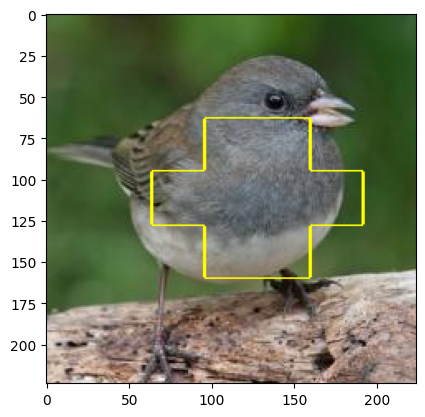
\includegraphics[width=.9\textwidth]{img/parameters/gradcam/threshold_05}
		\caption{Threshold 0.5}  \label{rys:parameters_lime_numsamples_1000}
	\end{subfigure}
	\begin{subfigure}[b]{0.45\textwidth}
		\centering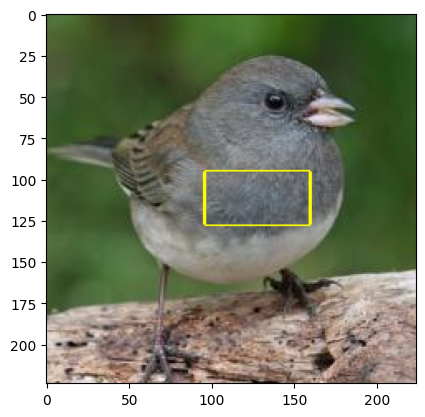
\includegraphics[width=.9\textwidth]{img/parameters/gradcam/threshold_09}
		\caption{Threshold 0.9}  \label{rys:parameters_lime_numsamples_1000}
	\end{subfigure}
	\caption{Przykład modyfikowania wyjaśnień GradCAM za pomocą threshold}

\end{figure}

\subsection*{Łączenie wyjaśnień}

Wyjaśnienia są łączone w tej pracy na 2 różne sposoby:
\begin{itemize}
	\item Część wspólna obszarów wyjaśnień (Rys. \ref{rys:example_combine_and}) - bardziej szczegółowe wyjaśnienia
	\item Suma obszarów wyjaśnień (Rys. \ref{rys:example_combine_or}) - bardziej ogólne wyjaśnienia
\end{itemize}

\begin{figure}[!h]
	\centering
	\begin{subfigure}[b]{0.45\textwidth}
		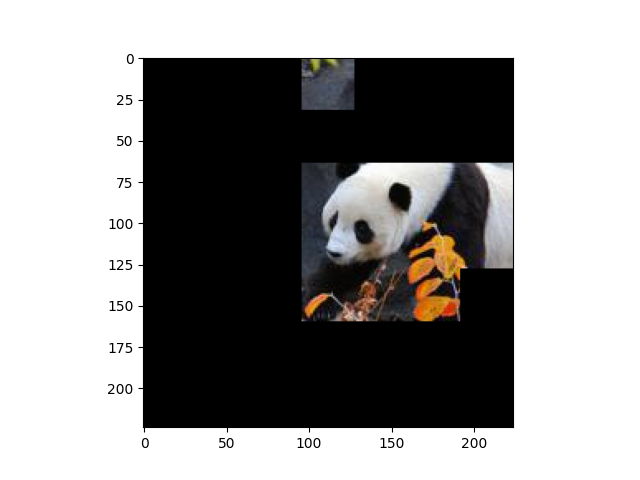
\includegraphics[width=.9\textwidth]{img/examples/first_explanation}
		\caption{Wyjaśnienie GradCAM}
	\end{subfigure}
	\begin{subfigure}[b]{0.45\textwidth}
		\centering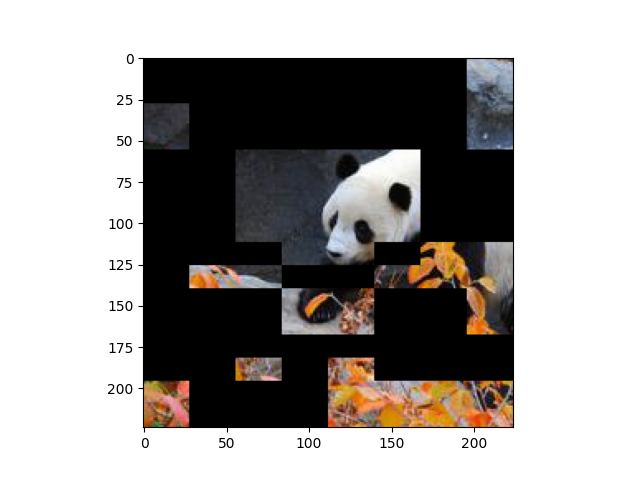
\includegraphics[width=.9\textwidth]{img/examples/second_explanation}
		\caption{Wyjaśnienie SHAP}
	\end{subfigure}
	\begin{subfigure}[b]{0.45\textwidth}
		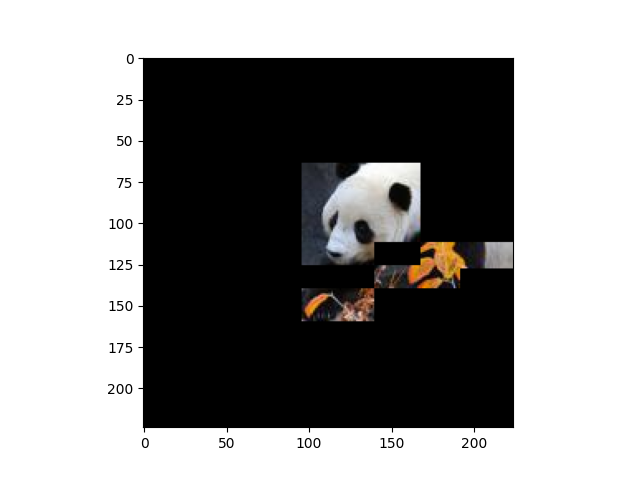
\includegraphics[width=.9\textwidth]{img/examples/and_explanation}
		\caption{Część wspólna wyjaśnień}  \label{rys:example_combine_and}
	\end{subfigure}
	\begin{subfigure}[b]{0.45\textwidth}
		\centering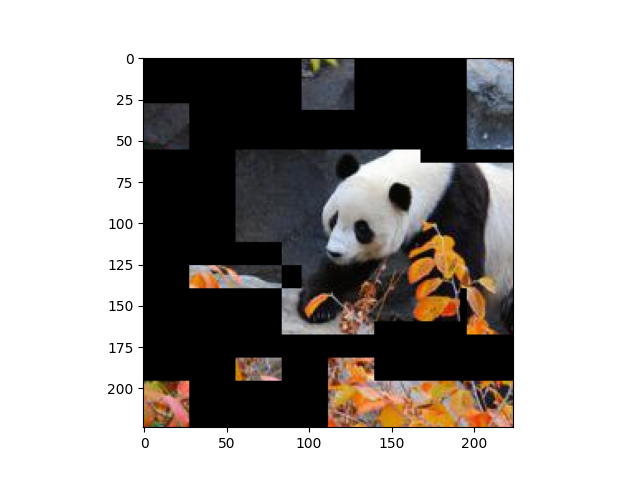
\includegraphics[width=.9\textwidth]{img/examples/or_explanation}
		\caption{Suma obszarów wyjaśnień}  \label{rys:example_combine_or}
	\end{subfigure}
	\caption{Przykład łączenia wyjaśnień}
\end{figure}

\section*{Miary jakości}

W tej sekcji skupiano się na opisie miar jakości, które zostały wykorzystane do oceny skuteczności metod wyjaśnialnej sztucznej inteligencji (XAI) w kontekście zadania klasyfikacji obrazów.

Wskaźnik \textbf{IoU} (Intersection ober Union), czyli stosunek przecięcia do sumy, jest powszechnie stosowany do pomiaru stopnia nakładania się dwóch obszarów.
W tej pracy, IoU jest używany do porównywania obszaru wyjaśnienia z obszarem rzeczywistego obiektu (informacje na ten temat pochodzą z ImageNet-9) oraz analizy spójności wyjaśnień.
Im wyższy IoU, tym lepiej wyjaśnienie pokrywa się z rzeczywistym obiektem na obrazie.
Wzór na IoU znajduje się w rozdziale 'Przegląd literatury' (\ref{eq:iou}).
Dodatkowo, wskaźnik IoU jest również używany do analizy spójności wyjaśnień, oceniając, w jakim stopniu różne metody wyjaśniania pokrywają te same obszary obrazu.

W celu oceny jakości wyjaśnień dodatkowo zbadano zmianę pewności modelu po modyfikacjach obrazu za pomocą wyjaśnień.

Badano \textbf{zmiany pewności po pozostawieniu samego obszaru wyjaśnienia} (Rys. \ref{rys:example_only_exp}).
Im lepsze wyjaśnienie, tym mniejszy powinien być średni spadek pewności (\ref{eq:average_drop}).
W pewnych przypadkach, gdy wyjaśnienie jest nadzwyczaj dobre, pewność modelu może nawet wzrosnąć, więc im dla większej części obrazów wzrasta pewność tym lepsza jest to metoda wyjaśniania (\ref{eq:rate_of-increase}).
Innymi słowy, im lepsze wyjaśnienie, tym większy procent przypadków, w których pewność modelu wzrosła po pozostawieniu obszaru wyjaśnienia.

\begin{figure}[h]
	\begin{subfigure}[b]{0.45\textwidth}
		\centering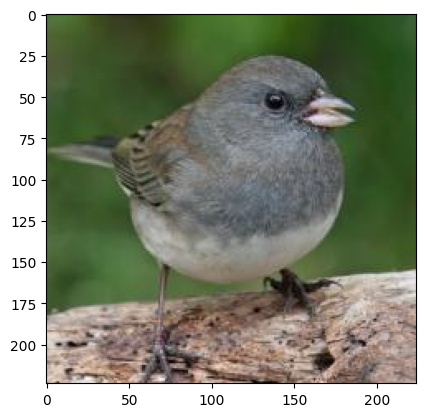
\includegraphics[width=.9\textwidth]{img/parameters/quality/base}
		\caption{Oryginalny obraz}
	\end{subfigure}
	\begin{subfigure}[b]{0.45\textwidth}
		\centering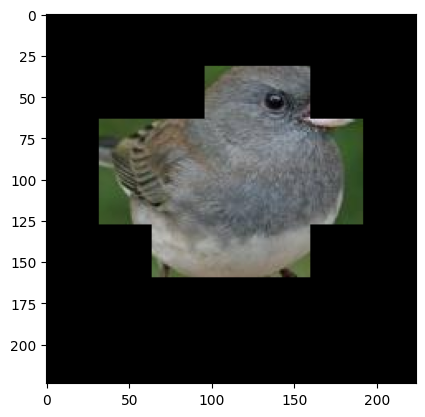
\includegraphics[width=.9\textwidth]{img/parameters/quality/mask}
		\caption{Sam obszar wyjaśnienia}
	\end{subfigure}
	\caption{Przykład pozostawienia samego wyjaśnienia}
	\label{rys:example_only_exp}
\end{figure}

Badano również \textbf{zmiany pewności po usunięciu obszaru wyjaśnienia} (Rys. \ref{rys:example_no_exp}) ocenia, jak zmienia się pewność modelu, gdy usunięty zostaje obszar wyjaśnienia.
Dobre wyjaśnienie powinno zaznaczać większość obszarów wpływających pozytywnie na pewność modelu, tak więc im większy średni spadek pewności tym lepsze jest to wyjaśnienie.

\begin{figure}[h]
	\begin{subfigure}[b]{0.45\textwidth}
		\centering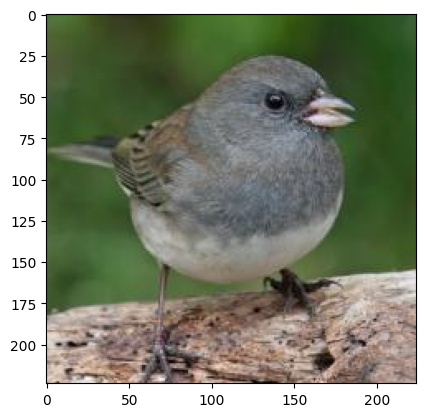
\includegraphics[width=.9\textwidth]{img/parameters/quality/base}
		\caption{Oryginalny obraz}
	\end{subfigure}
	\begin{subfigure}[b]{0.45\textwidth}
		\centering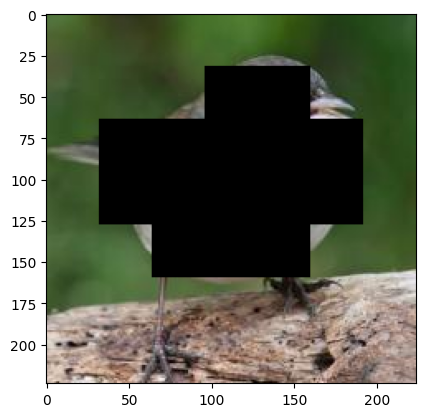
\includegraphics[width=.9\textwidth]{img/parameters/quality/wo_mask}
		\caption{Obraz bez obszaru wyjaśnienia}
	\end{subfigure}
	\caption{Przykład usunięcia obszaru wyjaśnienia}
	\label{rys:example_no_exp}
\end{figure}

